\documentclass[main]{subfiles}

\begin{document}

\chapter{Long reads assembly tools state of the art}\label{chapter:sota}

In previous chapter we see how we can clean data before run assembly. In this chapter we present methods to perform an assembly and how this methods was apply on long-read assembly tools we select this tools because method and algorithm used in it was representative how other tools work in addition, these tools are recognized by the community for their quality. We can see assembly tools can be split in step and between assembly we can found some similarity between step but we can observe in new assembly tools the steps can no longer be separated so easily.

\section{\textit{Greedy} assembly algorithm}

The \textbf{Greedy} assembly algorithm is the first type of assembly tools, used on Sanger data. For example, GigAssembler was used to assemble the first human genome data \cite{GigAssembler}. Algorithm \ref{intro:algo:greedy} present the global idea of how the \textbf{Greedy} algorithm work.

The BEST\_OVERLAP function is the main part of algorithm the best overlap is the larger one or the overlap with less error, each algorithm have her own choose method.

\begin{algorithm}[ht]
    \caption{A greedy assembly}
    \begin{algorithmic}[1]
    \Function{greedy}{reads}\Comment{reads is a set of read}
        \State choose r1 in reads
        \State sequence $\leftarrow$ r1
        \While{r2 $\leftarrow$ \Call{best\_overlap}{r1}}\Comment{\Call{best\_overlap}{\null} is a function for r1 they get read r2 the best overlap for read r1 in reads}
            \State \Call{concatenate}{sequence, r2}
            \State \Call{drop}{r1, reads}
            \State r1 $\leftarrow$ r2
        \EndWhile
    \EndFunction
    \end{algorithmic}
    \label{intro:algo:greedy}
\end{algorithm}

Moreover \textbf{Greedy} algorithm, by focusing on the local problem, weach overlap is the best one for this read, can't manage repetition. Genome contains many repetition, like a book some word are reused or complete part of sentence can be present multiple time.

Figure \ref{intro:fig:greedy:repetition} present a case where reads $R_0$ $R_1$ and $R_2$ contains a repetition. $R_0$ have two possible overlap if overlap with $R_1$ is choose the assembly sequence match with the green path, if overlap with $R_2$ is choose the assembly sequence match with the red path. We can't know which path is the good one and we didn't see the repetition. So assembly tools based on \textbf{Greedy} algorithm can produce many misassembly. 

\begin{figure}[ht]
    \centering 
    \subfile{introduction/tikz/repetition.tex}
    \caption{Each black box are a read, the grey box mark the position of a repetition. The begin of $R_1$ and $R_2$ are in repetition they share same begin but didn't match at her end. This repetition create a ambiguity in assembly.}
    \label{intro:fig:greedy:repetition}
\end{figure}

\subsection{Overlap Layout Consensus} \label{intro:subsec:OLC}

An alternative to the \textbf{Greedy} approach is the Overlap Graph Consensus (\OLC). We can find a first \OLC definition in \cite{OLC_myers} in 1995. The probably most popular assembly pipeline based on OLC is Celera \cite{celera_first, celera_second}. This approch is based on a graph where a read is a node and we build an edge between nodes if reads share an overlap. Figure \ref{intro:fig:olc:graph}, present the \OLC corresponding to ovelap present in \ref{intro:fig:greedy:repetition}.

We can see this graph like an ordering of pieces of book provided by a crazy copyist monk. An edge indicates that piece of text was before this piece of text in the original book.

The repetition creates a fork in \OLC, a node with two successor. It's easy to detect this case in the graph and stop this contig construction. The assembly result of this graph is 3 sequences with white node, green node and red node. The assembly is more fragmented than with the \textit{Greedy} algorithm but the assembly does not contain any misassembly.

\begin{figure}[ht]
    \centering 
    \subfile{introduction/tikz/overlap_graph.tex}
    \caption{Each node is a read and an edge is built between two read if they share an overlap.}
    \label{intro:fig:olc:graph}
\end{figure}

By analyzing the graph we will be able to detect the paths without branching node in the graph, and reconstruct the corresponding sequence by merging the sequences present in the graph.

\OLC based tools allow to avoid misassemblies but the search for overlap between reads is still expensive in time. The graph construction consumes a lot of memory, and more cleaning steps and graph analysis are expensive in computation time compared to a \textbf{Greedy} approach. 

\subsection{Algorithms and heuristics to simplify assembly graphs}

Graph structure was usefull to have complete view on all information provide by reads, but having too much information can create problems, slow down the assembly tools and increase their costs in memory or at worst lead to misassembly or to unnecessary fragmentation of the assembly.

\subsubsection{Transitive edge}  \label{intro:subsubsec:transitive_edge}

In Figure \ref{intro:fig:olc:graph} you can notice edge from $R_1$ to read $R_3$, this overlap was exact we can found an overlap between $R_1$ and $R_3$. But this edge didn't provides a new information we know $R_1$ is before $R_3$, this edge was call a transitive edge. More formally we can define a transitive edge, in a directed graph if we have this set of edge $(a, b)$ $(b, c)$ and $(a, c)$ the edge $(a, c)$ is transitive.

\citeauthor{string_graph} propose in \cite{string_graph} another assembly graph the \textbf{string graph} is an overlap graph without transitive edge. The string graph by reduce the number of edge in graph simplify traversing of the graph and memory impact of this one.

With string graph we just need follow simple path (path were all nodes have just one successor), to build assembly without misassembly.

\subsubsection{Contained reads} \label{intro:subsubsec:contained_reads}

In third generation technology, the crazy copyist monk provide fragment with different size and choose the begin of fragment randomly, so it's possible to have a read is contained in another one. All information (kmer or overlap with other reads) in contained reads was present in the container read for assembly task we can remove contained read, and save memory and time.

\subsubsection{Bubble and tips} \label{intro:subsubsec:bubble_tips}

We see how \OLC was build, but this construction step can include some specific structure, they can lead to misassemblies or fragmentation of assembly a cleaning step was required.

\begin{figure}[ht]
    \subfloat[][A example of tips in an assembly graph, the tips node wase represent in read, green, blue and black line underline different possible assembly scenario]{
        \subfile{introduction/tikz/cleaning_tips.tex}
        \label{intro:fig:cleaning:tips}
    }
    \subfloat[][A example of bubble in an assembly graph, each path was colored in different color. The length of each path can be different and we can have more than two path in bubble]{
        \subfile{introduction/tikz/cleaning_bubble.tex}
        \label{intro:fig:cleaning:bubble}
    }
    \caption{}
    \label{intro:fig:cleaning}
\end{figure}

A tips in an assembly graph is a node with only one edge, a tips can be create by many thing, trouble during DNA extraction, DNA duplication, sequencer create an artifact, a read with to many error ….

As we can see in Figure \ref{intro:fig:cleaning:tips} a tips can create a branching node in middle of simple path, if we keep this tips generally assembly create two contigs one before tips and one after tips (green and blue assembly scenario). If we remove this tips we can run the black scenario.

Its easy to detect and remove tips in graph, in many assembly tools tips are considered as errors and are removed.

We can define a bubble as a set of subpath in graph with same parent and same children, Figure \ref{intro:fig:cleaning:bubble} present an example with two path with same length. The bubble can be create by repetition or heterozygotie one or more version of this sequence contains a substitution or more complex mutation.

If bubble are large it can be harder to detect, with small bubble one version of the bubble are kept the choose of the version can be based on random choice or on coverage or other specific tricks.

\section{The advantages of long reads}

We say in Section \ref{section:introduction:sequencing} the main property of reads technology was length and error rate, the impact of error rate on read mapping and overlap search, was easy to understand, if reads contains many error it's harder to find the good mapping position and overlap.

Reads length have an very important impact on assembly quality \citeauthor{Bresler_Tse} in \cite{Bresler_Tse} introduce a notion of genome assembly \textbf{feasibility}, it's possible to reconstruct the genome from a reads set with this length and this coverage. To summarize very roughly, to get a good assembly reads need bridge must of repetion, so reads must be larger than the largest repetition. This idea was extend to reads with error in \cite{feasibility_with_error} and demonstrate we need increase coverage when error rate increase.

Before third generation sequencing the maximum length of read is lower than 2 kb (for Sanger read) or a majority of repetition in genome are larger than this length. \citeauthor{one_chromosome_one_contig} in \cite{one_chromosome_one_contig} indicate a theoretical length of read to obtain a perfect genome assembly for bacteria, read need to be upper than 7 kb, this limit not work in all practical case. If read are longer than repetition read can have a sufficient length before repetition cover all repetition and sufficient length after repetition we can solve the repetition see Figure \ref{intro:fig:whylongreads}.

\begin{figure}[ht]
    \centering
    \subfile{introduction/tikz/whyrepetition.tex}
    \caption{We have a part of assembly graph (\OLC or \DBG), node \texttt{R} represent a repetition node \texttt{A}, \texttt{B}, \texttt{C}, \texttt{D} represent basic sequence. Red, purple, green and blue line represent reads. Red read was larger than repetition and span over it and indicate $A_1 \rightarrow A_2 \rightarrow R \rightarrow C_1 \rightarrow C_2$ was a good path, with out this read we can solve this repetition.}
    \label{intro:fig:whylongreads}
\end{figure}

Third generation read aren't larger than all repetition but larger than many repetition and they help to produce better genome assembly. Table \ref{intro:tab:sr_lr_assembly} show improvement in term of N50 between short-read assembly and long-read assembly for some case. 

\begin{table}[]
    \centering
    \begin{tabular}{c|lll}
        Species & Short read N50 (bp) & Long read N50 (bp) & factor \\ \hline
        \textit{Gorilla gorilla gorilla} & 913,458 \cite{gorilla_sr_assembly} & 23,141,960 \cite{gorilla_genome} & 25 \\
        \textit{Schistosoma japonicum} & 176,869 \cite{s_japonicum_sr_assembly} & 1,093,989 \cite{s_japonicum_3rd_gene_improvement} & 6 \\
    \end{tabular}
    \caption{N50 scaffold of some genome assembly with short and long reads}
    \label{intro:tab:sr_lr_assembly}
\end{table}

Moerver \citeauthor{dnAQET} in \cite{dnAQET}, perform an assessment of different version of some wheel know assembly, \citeauthor{dnAQET} notice an important improvement in this assembly after introduction of third generation reads and 10X data (for more information on 10X data read Section \ref{section:other_contribution:10x}).

Recently a high quality human genome assembly (CHM13 cell line), telomere to telomere gaps less assembly, was produce with a combination of Nanopore and Pacbio reads \cite{telomere2telomere}. Author of this paper focus her effort on X chromosome, they reconstruct ~2.8 megabase centromeric satellite DNA array and closed all 29 remaining gaps in the current reference X \textit{H. sapiens} reference. Nanopore data by analysis of raw signal provide an access of DNA methylation this study confirm some previous epigenomic result observe X chromosome.

Long read technology not only help to improvement genome assembly. They also have a important impact in RNA study, sequencing mRNA from begin to end help to detect new isoform and splicing structure, by sequencing without PCR long reads help to remove bias in RNA quantification. But long read sequencing error rate and and large input material requirements (compared with short-read RNA-seq) require new analysis methodology development \cite{review_lr_rna}. 

After this overview of how \OLC assembly tools work, we going to details, two of long-read \OLC assembly tools, \canu and \miniasm.

\section{A Pipeline with correction \canu} \label{section:sota:canu}

Canu \cite{canu} was propose in 2016 is one of the first long reads assembly pipeline it's work with Pacbio and Nanopore reads after HGAP \cite{hgap}

\canu is based on \toolsname{Celera} \cite{celera_first, celera_second}, we can split the \canu pipeline in three steps, correction, trimming and assembly described below. Nevertheless, before each of these steps \canu search overlap between reads. We thus start by explaining how overlaps are computed.

\subsection{Overlapping} \label{subsec:sota:canu:overlapping}

In \canu pipeline overlap was compute by \mhap (for MinHash Alignment Process). We see previously found overlap between all reads take many time and required many memory. To avoid all versus all alignment \mhap try to estimate which read share a common part with another by estimate a Jaccard distance between the set of \kmers of two reads. The Jaccard distance, present in equation \ref{sota:equ:jaccard_dist} evaluate the distance between two set by divide the intersection of set by union of set.

\begin{equation}
J_{\delta}(A,B) = 1 - J(A,B) = 1 -  J(A,B) = 1 - \frac{|A \cap B|}{|A \cup B|}
\label{sota:equ:jaccard_dist}
\end{equation}

In this equation \texttt{A} and \texttt{B} represent the kmer set of read \texttt{A} and read \texttt{B}, if the $J(A,B)$ was low we can suppose read \texttt{A} and read \texttt{B} share a common part.
Enumerate all \kmers of each reads and compute intersection and union of each set take many times. \mhap select a subset of \kmers to represent the read and compute a mash distance \cite{mash_distance} see equation \ref{sota:equ:mash_dist_def} 

\begin{equation}
J(A,B) = \frac{|A \cap B|}{|A \cup B|} \approx \frac{|S(A \cup B) \cap S(A) \cap S(B)|}{|S(A \cup B)|}
\label{sota:equ:mash_dist_def}
\end{equation}

$S(A)$ is a \kmers set compose by $s$ first \kmers of set $A$. \citeauthor{mash_distance} evaluate the error between mash distance and Jaccard distance was in $\mathcal{O}(\frac{1}{\sqrt{s}})$, by default in \mhap $s=512$ so the error was smaller than 0.05.

In \mhap order \kmer with a \texttt{tf-idf} score, see equation \ref{sota:equ:tf_idf_def}. The \texttt{tf-idf} score come for text search domain. \texttt{tf-idf} evaluate if this term is specific to this document. \texttt{tf} for term frequency indicate if the term was present many times in document, $n_{i,j}$ how many time the term $i$ was present in document $j$ divide by the number of term in document $j$. \texttt{idf} for inverse document frequency evaluate if the term was present in many document or just in some document, $|\mathcal{D}|$ the number of document in dataset divide by $|\{d_{j}:t_{i}\in d_{j}\}|$ the number of document where the term $i$ was present.

\begin{equation}
\mathrm{tf-idf_{i,j}} = \mathrm{tf_{i,j}} \cdot \mathrm{idf_{i}} = \frac{n_{i,j}}{\sum_{k}n_{k,j}} \cdot \log{\frac  {|\mathcal{D}|}{|\{d_{j}:t_{i}\in d_{j}\}|}}
\label{sota:equ:tf_idf_def}
\end{equation}

In \mhap term was \kmer and document was read, this technique permit to reduce the number of \kmer in set and keep \kmer specific to a read. If two read share specific \kmer they probably share a common part.

If two reads have a small mash distance \mhap compare the position of each \kmer in reads to determinate the overlap position.

The size of \kmer was very important to if k is too large many \kmer contains error the size of intersection was reduce and \mhap can miss overlap. Moreover size of sketch have a huge impact if it's to small the read was sub-sample if it's to large compute mash distance take more time, but with long-reads dataset the length of reads can be very different choose a good sketch size for this type of data isn't easy. To found optimal value of this two variable authors of \mhap perform many empirical test.

\subsection{Correction}

In \canu correction was performed by a part of \toolsname{FALCON} \cite{falcon}, \toolsname{falcon\_sense}. \toolsname{FALCON} and \canu was develop simultaneously, we choose to describe \canu in detail in place of \toolsname{FALCON} because we work principaly with \canu. In this section we didn't present in details how \toolsname{falcon\_sense} work but only the main idea.

Some correction tools as \toolsname{falcon\_sense} use a Partial Order Alignment (POA) (introduce in \cite{poa}) to perform long read correction. For each read \texttt{$R_1$} we recruit all read share an overlap with him, and perform an exact alignment with him. This alignment was use to build a POA graph, in POA graph each base was a node and a direct edge was create between two base if the first base was before the second one in an alignment. If an edge was present in two alignment her weight was increment. After all alignment was add in the POA graph, we search weighed path in this graph, and follow to reconstruct the corrected sequence. An example of POA graph construction was present in figure \ref{sota:fig:canu:correction}

\begin{figure}[ht]
    \centering
    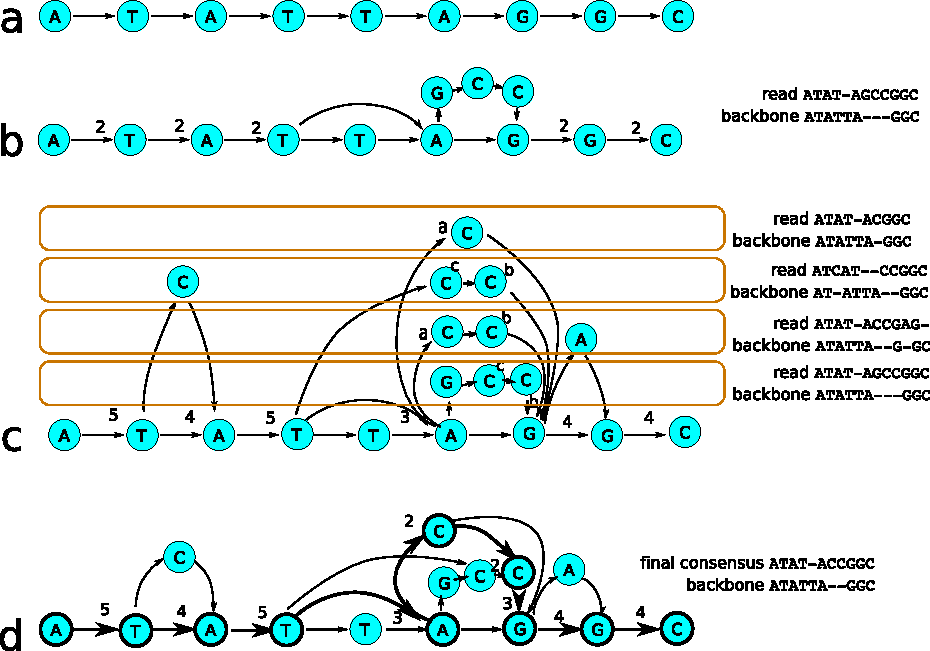
\includegraphics[width=\textwidth]{state_of_the_art/images/POA_explain.pdf}
    \caption{Sequence need to be correct was represent as a graph, each base was a node and if a base is follow by another an directed edge was build. (b) was the representation of sequence \texttt{ATATTAGGC} (call backbone in this figure), (b) We add the result of alignment of one read in the graph, number upper than edge was her weigth if and edge exist in some 3 alignment her weight was egal to 3, (c) We add all other alignment in the graph, (d) the bold path was choose a the correct path because it was supported by more alignment. This figure was originaly present in Supplementary material of \hgap \cite{hgap}}
    \label{sota:fig:canu:correction}
\end{figure}

\subsection{Trimming}

The trimming step will remove the parts of the reads that are not supported by the other reads, see Figure \ref{sota:fig:canu:trimming}. For each reads we will analyze its coverage curve and remove the parts of the reads that are not sufficiently covered (by default this value is set to 1), for trimming \canu use an homemade tools. 


\begin{figure}[ht]
    \centering
    \subfile{state_of_the_art/tikz/trimming.tex}
    \caption{Black arrow line was the path choose by \canu, the other line was a reads mapped against this path, the blue box indicate a repeat region. In case \texttt{A} the purple read span all the repetition and indicate that the path choose by \canu was the good one. In case \texttt{B} no read span the repetition, and the purple read have some not congruent overlap between red and blue read, so \canu need break the path to didn't create a misassembly}
    \label{sota:fig:canu:trimming}
\end{figure}

\subsection{Assembly}

\canu assembly step is based on \OLC paradigm (see Section \ref{intro:subsec:OLC} for \OLC definition), with some specificity. \canu build a Best Overlap Graph (BOG) for each not contained read only two overlap are kept in the graph, the best overlap for each read extremity, in \canu the best overlap was the longest overlap. Usage of a BOG in place of classic \OLC graph is an aggressive strategy, in BOG we can't observe a transitive edge and the number of edge was equal bound by the number of node. We avoid a cleaning step and reduce the memory impact of the graph. After this graph construction step performed, some clean step was run, remove tips and little buble (see Section \ref{intro:subsubsec:bubble_tips}).

This BOG was used as a scaffold to generate assembly, by remapping read against this scaffold, \canu try to detect repetition, larger than read not show in BOG as loop, and to call read to build a consensus after. Each simple path in BOG was used to build a contig. 

By remapping reads on the BOG \canu can build a consensus and detect repetition didn't observe in graph. BOG was an aggressive strategy to avoid transitive edge and reduce graph size but they can mask an edge denote a repetition this check was required to.

\begin{figure}[ht]
    \centering
    \subfile{state_of_the_art/tikz/BOG_remapping.tex}
    \caption{Black line was a reads, the \canu trimming step keep only the blue part of read $R_0$, part covered by other read.}
    \label{sota:fig:canu:remapping}
\end{figure}

\section{Pipeline without correction \miniasm} \label{section:sota:miniasm}

\minimap and \miniasm was an assembly pipeline proposed in \cite{miniasm_minimap} and \cite{minimap2}, the main purpose of this pipeline is to demonstrate we can perform a long read assembly without correct long read before.

The miniasm pipeline is simpler than the canu pipeline because it does not incorporate correction and consensus building. It is composed by steps:
\begin{itemize}
    \item overlap search, performed by minimap
    \item trimming, by miniasm
    \item graph construction 
    \item graph cleaning
    \item contig generation
\end{itemize}


\subsection{\minimap} \label{subsec:sota:miniasm:minimap}

Main idea to \minimap (similar to \mhap) is we can represent a read as a set of some minimal kmer, and if two read share same succession of minimal kmer we can suppose this two read share an overlap.

A minimal kmer is a the kmer for a set of consecutive kmer than minimize her score, the score function was the same during all analyse and for the same set of consecutive kmer the same kmer was the minimizer. Moreover a kmer can be minimizer of some consecutive set of kmer, if no other kmer with lowest score come in window. 

\begin{figure}[ht]
    \centering
    \subfile{state_of_the_art/tikz/minimizer.tex}
    \caption{The red kmer have the lowest score of the red window so it's the minimizer of this window. But when window slice on the blue kmer this one have a lowest score, the blue kmer become the minimizer of this window.}
    \label{sota:fig:miniasm:minimizer}
\end{figure}

The minimal \kmer can represent many other read, this technique can be compare to a loosly compression.

\minimap build an index where each minimizer are associate to reads where minimizer is present and position of this minimizer in reads.

With this index \minimap can collect position of similar minimizer between two reads, with this collection of position \minimap search the largest co-linear match, a succession of similar minimizer in each reads with coherent position, same order of minimizer and similar distance between each minimizer. Figure \ref{sota:fig:miniasm:mapping} show an overview of a overlap of two reads in \minimap.

\begin{figure}[ht]
    \centering
    \subfile{state_of_the_art/tikz/minimap.tex}
    \caption{$Read_A$ and $Read_B$ was represent by black arrow. Common minimizer of $Read_A$ and $Read_B$ was represent by blue and red arrow respectively. Green arrow was a co-linear chain, purple arrow was another co-linear chain, black arrow didn't participate to a co-linear chain. The longest colinear chain was the green one the end of $Read_A$ probably overlap the begin of $Read_B$.}
    \label{sota:fig:miniasm:mapping}
\end{figure}

\minimap report overlap where the number of match is sufficient (upper than a threshold) and  total length of putative overlap was sufficient. 

\subsection{\miniasm}

\miniasm didn't perform correction but they didn't take all information from reads and overlap, some filtering operation was performed.

For each read \miniasm perform coverage analysis of reads based on mappings identify by \minimap, by default only the longest part of reads with a coverage upper than three are kept. \minimap report for each read, read length, position of first and last kmer, number of bases in kmer exact match,  and a mapping quality and some option field in SAM like format can be present too.

\begin{figure}[ht]
    \centering
    \subfile{state_of_the_art/tikz/miniasm_overlap.tex}
    \caption{\miniasm classify overlap in three type of dovetail, internal match and containment overlap. Black grey region correspond to part of read between first and last minimizer. Light grey region was called overhang region, it's out of minimizer range. If overhang was large compare to overlap region we can supects this overlap isn't a true overlap.}
    \label{sota:fig:miniasm:ovl_classification}
\end{figure}

Each overlap was classified in three category, in order to keep only true end-to-end overlap to build the \OLC and filter out containment reads:
\begin{itemize}
    \item internal match, this type of overlap probably correspond to a repetition smaller than reads length
    \item containment, a read of this overlap was contains in the other read it's same sequence
    \item dovetails, it's a end-to-end overlap
\end{itemize}
Figure \ref{sota:fig:miniasm:ovl_classification} show some example of this overlap. Containment read was removed, only dovetail overlap was used to build overlap graph. Tips, small bubble and transitive edge was removed after this step \miniasm take each simple path and concatenate substring of read between begins and the first position of overlap.

\miniasm was design to work on uncorrected read and didn't perform a consensus step so contigs generate by \miniasm contains many error and can't be used directly. We can run \minimap \miniasm pipeline with corrected read and a polishing tools on contig generate by \miniasm. 

Very recently, another assembly tool \toolsname{Ra}\cite{Ra} was a create to replace \miniasm in \minimap \miniasm pipeline. \toolsname{Ra} use an analysis of coverage curve of each reads to trim not supported region like \miniasm but they include the detection of chimera and repeat region. Overlap on region marked as repeat are marked in string graph and not trusted. \toolsname{Ra} perform a real consensus step and run many polishing step with \toolsname{Racon}. According to the authors and another study\cite{long_read_assembler_comparison}, Ra performs good assembly on bacteria and plant genome assembly the overlap step still can be optimize in term of memory usage and computation time.

\section{\DBG like long reads assembly approach} \label{section:sota:wtdbg}

\DBG tools try to speed up assembly by simplify the overlap search step. This method was proposed in \toolsname{EULER} \cite{eulerian_approach}.

This approach is based on a DeBruijn Graph (or \DBG). For an alphabet with $n$ symbols a \DBG represents each word of length $k$ as node and builds a directed edge if node share $k - 1$ symbol at them extremities. For example, in Figure \ref{intro:fig:dbg:graph}, node \texttt{ATCG} and \texttt{TCGG} share \texttt{TCG}. A word of length $k$ is called a \kmer.

In assembly problems, $n = 4$ (${A, C, T, G}$), and we can choose a value of k between 1 and the read length. In practice, this size is often smaller than the size of a read the choice of the right values of k, depending on the use that we will have of the \DBG could be the subject of a complete thesis.

To build the \DBG we choose a value of $k$ and we add all \kmer present in reads in the \DBG. The \DBG used in assembly contains only \kmer present in dataset not all possible \kmer, and edge can be only edge present in dataset or all possible edges.

\begin{figure}[ht]
    \center
    \subfile{introduction/tikz/debruijn_graph.tex}
    \caption{We have a dataset of 4 reads with length equal to 7, we choose a value equal to 4, kmer was present under each read. A \DBG build from this kmer set was present under kmer, each node was a kmer and if a word share $k - 1$ symbol at is end with $k - 1$ symbol at begin of another node we build a directed edge. This \DBG contains cycle this cycle probably match with a repetition in original sequence}
    \label{intro:fig:dbg:graph}
\end{figure}

Like \OLC we can detect repetition by inspect the number of successor of a node Figure \ref{intro:fig:dbg:graph} present a \DBG with a repetition. After build the \DBG we can follow the simple path to rebuild the original sequence.

With \DBG strategy we didn't compute overlap between reads, but the length of word in graph was shorter. And all repetition with a size upper than $k$ create cycle in the graph and fragment the assembly.

Moreover the overlap between word in \DBG must exact (without error) and with a fixed length ($k - 1$), these two constraints are particularly problematic when the reads contain a lot of error or when the coverage of the region is low.

\DBG approach was used succesfly for short-read assembly we can cite tools \toolsname{Spades} \cite{spades}, \toolsname{Minia} \cite{minia} and \toolsname{Megahit}\cite{megahit} but this technics isn't very efficient for long reads assembly:
\begin{itemize}
    \item reads contain a high error rate and therefore found error-free kmers was hard, this error can lead to expand size of graph and or mis-connection between part of graph.
    \item size of kmer was generaly lower than 100 base and manage larger kmer was hard without usage of many memory, moreover \DBG can't manage repetition larger kmer.
\end{itemize}

If we use \DBG naively for long read assembly, we can mis the main advantage of long-reads her length.

\flye and \wtdbg use \DBG approach with some modification to adapt this idea to long-read assembly. \flye create a A-Bruijn Graphs(\abreviation{ABG}), where edge didn't denote an overlap with length k-1 between node but the overlap can be shorter. In \wtdbg method kmer was replace by k-bin where a bin was a substring (256 bases of length by default) of reads, and are generate between k-bin if they are successive in a reads.

\subsection{\flye}

\flye\cite{Flye} was based on \abruijn\cite{abruijn} assembly tools. \abruijn didn't use a \DBG but a similar concept a \abreviation{ABG}, in place of use a set of kmers as node \abreviation{ABG} use a set of chosen kmers, in place of build an edge between each kmer they share a k-1 overlap they build an edge with a weight equal to the distance of kmer in the original string between without create transitive edge.

To build the chosen \kmers set, \abruijn select kmers present many times in dataset this kmers was called in many tools \textit{solid} \kmers \jsv{citer le papier qui introduit la notion de solid kmer} \pim{Sa existe ? demander a Rayan}. The more a \kmers is present in the dataset, the more sure you may be that this \kmers does not contain a sequencing error, if the genome coverage is 40x we can hope see \kmer, not include in a repetition, 40 times. Because when we sequence at 40x we didn't really read each base 40 times and when a sequence error appear we lost an occurrence of the kmers where this base was present, choose the number of times a kmer need to be present in dataset to be \textit{solid} was an hard task.

This modification help to clean sequencing error, but reduce the set of kmer fragment \DBG graphes it's why \abreviation{ABG} create edge not only when kmers share k-1 overlap. 

During the \abreviation{ABG} construction \abruijn store wich read generate wich graph path, this structure was usefull to found speedly overlap between reads. Reads participate to the same path of \abreviation{ABG} have probably the same sequence so they probably share an overlap. To build contigs \abruijn take a read $R_1$ found all overlap with help of \abreviation{ABG} if this local overlap graph didn't denote a fork, we have one read without successor and all reads have path in graph to this read, \abruijn extend the contig.

\abruijn can be roughly resume as mix of all assembly strategy, use \DBG to found overlap between read, build contigs by extension like \textit{greedy} methode but use \OLC to check they aren't integrate a repetition and a potential missassembly in contigs.

\flye was build on top of \abruijn, after \abruijn assembly \flye search self alignment in assembly. If extremity of contig are similar they are tag as repetition. \flye build a repetition graph, where repetition extremity as node and a edge was build when to repetition extremity was link in a contig. \flye use coverage information to take a clue on contig succession over untangle repetition. By analysis the topology of repetition graph \flyecan found a uniq traversal path to explain all repetition and found the genomic order of contig.

\subsection{\wtdbg}

\wtdbg \cite{wtdbg2}  use a \DBG approch to solve long-read assembly, isn't realy a \DBG but a "Fuzzy-Brujin graph" (\abreviation{FDBG}) firstly define in this paper. To build this graph \wtdbg split read in bin with a fixed size (256 base pairs) and they store kmer present in each bin in a hash table.
To find overlap between reads wtdg2 use an hash table to compare the kmer composition between each reads and perform an exact alignment between each bin of reads. 

After this alignment step \wtdbg keep only in memory wich bin are align to which bin, and they build a k-bins each k-bins is a sequence of k successive bin in a read, \wtdbg can infer if two k-bins overlap if some bin in this two k-bins share an ovelap.

A group of k-bins are a node of \abreviation{FDBG}, \wtdbg build an edge between two node if a k-bins in each node are succesive in a read, after some cleanning step (pops bubbles, tips cleanning) \wtdbg build a consensus sequence with each simple path in \abreviation{FDBG}.

\section{New long read assembly method}

Very Recently two assembly tools was present this focus on capability to product good long read assembly with a very low cost in computation time and memory usage.

\subsection{Peregrine}

\newcommand{\shimmer}{\toolsname{SHIMMER}}

\peregrine \cite{Peregrine} use \shimmer overlapper. \shimmer extend idea of minimizer (present in Section \ref{subsec:sota:miniasm:minimap}), by create minimizer of minimizer. A minimizer can represent a set of minimizer these minimizers representing a set of kmer, we can had many layer of minimizer, each layer reduce the size of minimizer set and space of search to found similarity between reads.

The layer-0 of minimizer was a basic minmizer process, like \minimap. After this step \shimmer, select minimizer they participate to the layer-1, they use a reduction factor, for a reduction factor $x$, $x$ minimizer was represent by the minimal minimizer of this set, this process can be repeat with many layer. When they choose the minimizer of $layer_n$ minimizer of $layer_{n-1}$ \shimmer take care of distance between each $layer_n$ minimizer to be shure they represent a distinct part of the read.  \shimmer by default use three layer of minimizing this value, reduce the number of minimizer need to be compare to found similarity, without increase the number of overlap missed (value found empiricaly).

After this indexing step, \shimmer group reads they share many minimizer of last layer and perform a classic alignment to confirm overlap between reads. After this step \peregrine run a classic \OLC strategy to perform assembly.

\shimmer overlapping tools can be use to perform a mapping of read against contig or genome, after this remapping a poolshing step was perform, without a take an account to heterozygotie.

\peregrine was actually test only Circular Consensus (CCS) Pacbio data. Reads was sequence multiple time and a consensus was perform on all this sequencing, this technique reduce length of read but reduce the error level of sequencing too. Found overlap between reads with less error was easier and faster. Methods create by \peregrine tools by reducing the minimizer space of search seedup the search of overlap, but they was test on low error rate long reads, even if the error rates of long reads try to decrease, will they decrease sufficiently for this method to maintain a good sensitivity. \peregrine need to be validate on other type of data before her method be generalize.

\subsection{Shasta}

\newcommand{\shasta}{\toolsname{Shasta}}

\shasta was recently publish assembly tools they was used to assembly Nanopore data of eleven human genome \cite{Shasta}.

\shasta use read-length representation of reads, read-length representation was a loss-less compression method for text was contains a large repetition of same character. For example sequence \texttt{ACCTTTGAA}, was represent by two string $Sb$ \texttt{A C T G A} and $St$ \texttt{1 2 3 1 2}. To reconstruct original sequence we repeat $St_i$ time the $Sb_i$ letre.

This representation was interesting for long-reads data, because DNA contains sometimes same character repetition (called an homopolymer) and long-reads make many times error in homopolymer, read-length representation by squashing this region can avoid this type of error, and facilitate alignment of long-reads.

To perform read overlapping \shasta, didn't use a minimizer approach but something very close, the $Sb$ string of read was split in kmer and some kmer was selected randomly, and called marker, the set of marker was the same for all data set. Reads was now represent by a succession of marker it's a lossly compression.

Before search a colinear match of marker, to select reads with higher probability of match \shasta compute a modification of MiniHash Jaccard estimation (see Section \ref{subsec:sota:canu:overlapping}) to avoid bias create by difference of length between reads.

To perform assembly \shasta create a marker graph, it's something similar to \DBG, where kmer was marker and an edge was build between two marker if a read contains this succession of marker, each edge was weighted by the number of reads they contains this succession, after a cleaning step of marker graph (removing transitive edge, tips and bubble) path in marker graph was select and reads participate to building of edge of this path was used to build a consensus sequence of contigs.

\shasta contains many interesting idea and author's plan some improvement for heterozygotie detection, resolution and performance improvement.

\section{Chapter Conclusion}

Long read assembly was an active field of search many tools was create each year, and long read assembly tools was used to improve genome and build draft genome.

To perform overlap detection a majority of tools use k-mer, to found reads with an high similarity and avoid all-versus-all overlapping search. To further reduce the space search some tools filtering based on minimizing, we keep kmer with the lowest score, this score can be based on information contains in dataset or be determinate by an arbitrary function. The choose of k-mer size, filtering method, minimizing function, can have many impact on result of each tools. 

The \OLC approach has proven its effectiveness in assembling third generation reads. Several modifications have been made to support these new reads but efforts are mainly focused on reducing the computation time of memory usage. This modification lead to hybrid \OLC algorithm with \DBG and Greedy, (cf \flye and \wtdbg) idea. But the step this take the most time and memory isn't the graph construction and contig construction but search of overlap and the correction.

Isn't only the challenge need to be address, many assembly step have important cost in computation time and memory usage. For exemple get an overlap search with high precision and recall and without excessive cost in computation time and memory usage \cite{bench_ovl}.

The only one assembly they try to take in account heterozygotie was \toolsname{FALCON}, and in future \shasta, make difference between an sequencing error and a natural variant or heterozygotie. Get heterozygotie and variant phased or genome graph after assembly was interesting. But tools to extract all this information from read didn't exist yet

Another step of assembly improvement was increase the contiguity, assembly tools by reduce the information to reduce computation time and memory usage can have an effect on assembly quality. Correction of long-read can by trimming unsuffisent covered data can increase the size of coverage gap.
By come back to all read information or use overlap found by another tools, help to solve assembly trouble, create by heuristic in assembly and correction tools. The next chapter are focus on this points.


\onlyinsubfile{
\bibliographystyle{plainnat}
\bibliography{main}
\addcontentsline{toc}{chapter}{Bibliography}
}

\end{document}